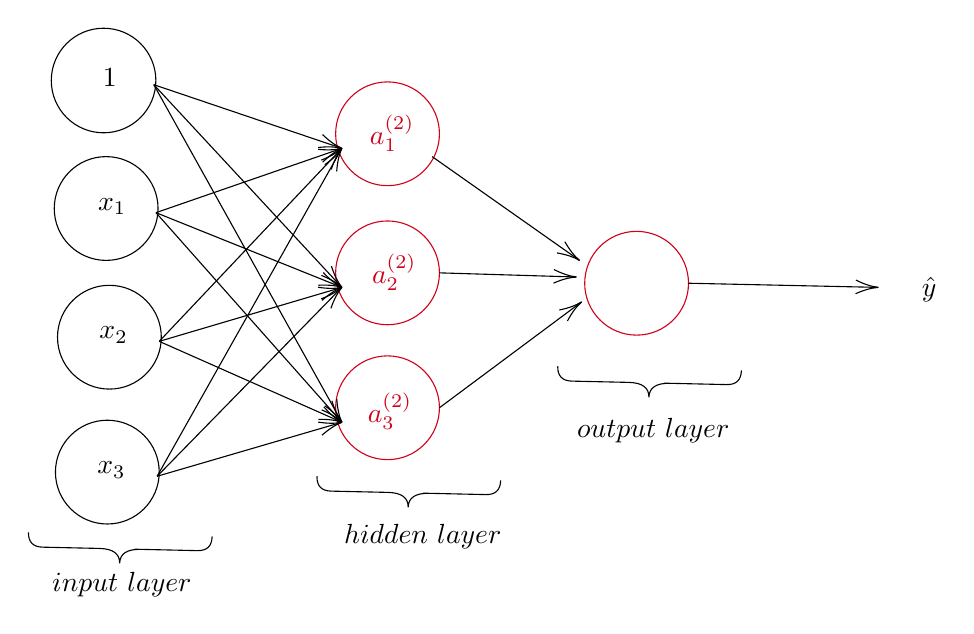
\begin{tikzpicture}[x=0.75pt,y=0.75pt,yscale=-1,xscale=1]
%uncomment if require: \path (0,300); %set diagram left start at 0, and has height of 300

\draw  [color={rgb, 255:red, 208; green, 2; blue, 27 }  ,draw opacity=1 ]  (241, 71) circle [x radius= 25, y radius= 25]  ;
\draw  [color={rgb, 255:red, 208; green, 2; blue, 27 }  ,draw opacity=1 ]  (241, 138) circle [x radius= 25, y radius= 25]  ;
\draw  [color={rgb, 255:red, 208; green, 2; blue, 27 }  ,draw opacity=1 ]  (241, 203) circle [x radius= 25, y radius= 25]  ;
\draw    (262.5,82) -- (333.5,132) ;
\draw [shift={(333.5,132)}, rotate = 215.15] [color={rgb, 255:red, 0; green, 0; blue, 0 }  ]   (0,0) .. controls (3.31,-0.3) and (6.95,-1.4) .. (10.93,-3.29)(0,0) .. controls (3.31,0.3) and (6.95,1.4) .. (10.93,3.29)   ;

\draw    (266,138) -- (332,140) ;
\draw [shift={(332,140)}, rotate = 181.74] [color={rgb, 255:red, 0; green, 0; blue, 0 }  ]   (0,0) .. controls (3.31,-0.3) and (6.95,-1.4) .. (10.93,-3.29)(0,0) .. controls (3.31,0.3) and (6.95,1.4) .. (10.93,3.29)   ;

\draw    (266,203) -- (334.5,152) ;
\draw [shift={(334.5,152)}, rotate = 503.33] [color={rgb, 255:red, 0; green, 0; blue, 0 }  ]   (0,0) .. controls (3.31,-0.3) and (6.95,-1.4) .. (10.93,-3.29)(0,0) .. controls (3.31,0.3) and (6.95,1.4) .. (10.93,3.29)   ;

\draw  [color={rgb, 255:red, 208; green, 2; blue, 27 }  ,draw opacity=1 ]  (361, 143) circle [x radius= 25, y radius= 25]  ;
\draw    (386,143) -- (477.5,145) ;
\draw [shift={(477.5,145)}, rotate = 181.25] [color={rgb, 255:red, 0; green, 0; blue, 0 }  ]   (0,0) .. controls (3.31,-0.3) and (6.95,-1.4) .. (10.93,-3.29)(0,0) .. controls (3.31,0.3) and (6.95,1.4) .. (10.93,3.29)   ;

\draw    (105.43, 107) circle [x radius= 25, y radius= 25]  ;
\draw    (107, 169) circle [x radius= 25, y radius= 25]  ;
\draw    (106, 234) circle [x radius= 25, y radius= 25]  ;
\draw    (104.19, 45.33) circle [x radius= 25.19, y radius= 25.19]  ;
\draw    (128.38,47.33) -- (219,78) ;
\draw [shift={(219,78)}, rotate = 198.7] [color={rgb, 255:red, 0; green, 0; blue, 0 }  ]   (0,0) .. controls (3.31,-0.3) and (6.95,-1.4) .. (10.93,-3.29)(0,0) .. controls (3.31,0.3) and (6.95,1.4) .. (10.93,3.29)   ;

\draw    (128.38,47.33) -- (219,145) ;
\draw [shift={(219,145)}, rotate = 227.14] [color={rgb, 255:red, 0; green, 0; blue, 0 }  ]   (0,0) .. controls (3.31,-0.3) and (6.95,-1.4) .. (10.93,-3.29)(0,0) .. controls (3.31,0.3) and (6.95,1.4) .. (10.93,3.29)   ;

\draw    (128.38,47.33) -- (219,210) ;
\draw [shift={(219,210)}, rotate = 240.88] [color={rgb, 255:red, 0; green, 0; blue, 0 }  ]   (0,0) .. controls (3.31,-0.3) and (6.95,-1.4) .. (10.93,-3.29)(0,0) .. controls (3.31,0.3) and (6.95,1.4) .. (10.93,3.29)   ;

\draw    (129.43,109) -- (219,210) ;
\draw [shift={(219,210)}, rotate = 228.43] [color={rgb, 255:red, 0; green, 0; blue, 0 }  ]   (0,0) .. controls (3.31,-0.3) and (6.95,-1.4) .. (10.93,-3.29)(0,0) .. controls (3.31,0.3) and (6.95,1.4) .. (10.93,3.29)   ;

\draw    (129.43,109) -- (219,145) ;
\draw [shift={(219,145)}, rotate = 201.9] [color={rgb, 255:red, 0; green, 0; blue, 0 }  ]   (0,0) .. controls (3.31,-0.3) and (6.95,-1.4) .. (10.93,-3.29)(0,0) .. controls (3.31,0.3) and (6.95,1.4) .. (10.93,3.29)   ;

\draw    (129.43,109) -- (219,78) ;
\draw [shift={(219,78)}, rotate = 520.9100000000001] [color={rgb, 255:red, 0; green, 0; blue, 0 }  ]   (0,0) .. controls (3.31,-0.3) and (6.95,-1.4) .. (10.93,-3.29)(0,0) .. controls (3.31,0.3) and (6.95,1.4) .. (10.93,3.29)   ;

\draw    (131,171) -- (219,78) ;
\draw [shift={(219,78)}, rotate = 493.42] [color={rgb, 255:red, 0; green, 0; blue, 0 }  ]   (0,0) .. controls (3.31,-0.3) and (6.95,-1.4) .. (10.93,-3.29)(0,0) .. controls (3.31,0.3) and (6.95,1.4) .. (10.93,3.29)   ;

\draw    (131,171) -- (219,145) ;
\draw [shift={(219,145)}, rotate = 523.54] [color={rgb, 255:red, 0; green, 0; blue, 0 }  ]   (0,0) .. controls (3.31,-0.3) and (6.95,-1.4) .. (10.93,-3.29)(0,0) .. controls (3.31,0.3) and (6.95,1.4) .. (10.93,3.29)   ;

\draw    (131,171) -- (219,210) ;
\draw [shift={(219,210)}, rotate = 203.9] [color={rgb, 255:red, 0; green, 0; blue, 0 }  ]   (0,0) .. controls (3.31,-0.3) and (6.95,-1.4) .. (10.93,-3.29)(0,0) .. controls (3.31,0.3) and (6.95,1.4) .. (10.93,3.29)   ;

\draw    (130,236) -- (219,78) ;
\draw [shift={(219,78)}, rotate = 479.39] [color={rgb, 255:red, 0; green, 0; blue, 0 }  ]   (0,0) .. controls (3.31,-0.3) and (6.95,-1.4) .. (10.93,-3.29)(0,0) .. controls (3.31,0.3) and (6.95,1.4) .. (10.93,3.29)   ;

\draw    (130,236) -- (219,145) ;
\draw [shift={(219,145)}, rotate = 494.36] [color={rgb, 255:red, 0; green, 0; blue, 0 }  ]   (0,0) .. controls (3.31,-0.3) and (6.95,-1.4) .. (10.93,-3.29)(0,0) .. controls (3.31,0.3) and (6.95,1.4) .. (10.93,3.29)   ;

\draw    (130,236) -- (219,210) ;
\draw [shift={(219,210)}, rotate = 523.72] [color={rgb, 255:red, 0; green, 0; blue, 0 }  ]   (0,0) .. controls (3.31,-0.3) and (6.95,-1.4) .. (10.93,-3.29)(0,0) .. controls (3.31,0.3) and (6.95,1.4) .. (10.93,3.29)   ;

\draw   (68,263) .. controls (67.89,267.67) and (70.17,270.05) .. (74.84,270.16) -- (102.1,270.77) .. controls (108.76,270.92) and (112.04,273.32) .. (111.93,277.99) .. controls (112.04,273.32) and (115.42,271.07) .. (122.09,271.22)(119.09,271.15) -- (149.34,271.83) .. controls (154.01,271.94) and (156.39,269.66) .. (156.5,264.99) ;
\draw   (207,236) .. controls (206.89,240.67) and (209.17,243.05) .. (213.84,243.16) -- (241.1,243.77) .. controls (247.76,243.92) and (251.04,246.32) .. (250.93,250.99) .. controls (251.04,246.32) and (254.42,244.07) .. (261.09,244.22)(258.09,244.15) -- (288.34,244.83) .. controls (293.01,244.94) and (295.39,242.66) .. (295.5,237.99) ;
\draw   (323,183) .. controls (322.89,187.67) and (325.17,190.05) .. (329.84,190.16) -- (357.1,190.77) .. controls (363.76,190.92) and (367.04,193.32) .. (366.93,197.99) .. controls (367.04,193.32) and (370.42,191.07) .. (377.09,191.22)(374.09,191.15) -- (404.34,191.83) .. controls (409.01,191.94) and (411.39,189.66) .. (411.5,184.99) ;

\draw (243.21,70.84) node [color={rgb, 255:red, 208; green, 2; blue, 27 }  ,opacity=1 ]  {$a^{( 2)}_{1}$};
\draw (244.21,137.84) node [color={rgb, 255:red, 208; green, 2; blue, 27 }  ,opacity=1 ]  {$a^{( 2)}_{2}$};
\draw (242.21,204.84) node [color={rgb, 255:red, 208; green, 2; blue, 27 }  ,opacity=1 ]  {$a^{( 2)}_{3}$};
\draw (109,168) node   {$x_{2}$};
\draw (108.37,105.96) node   {$x_{1}$};
\draw (108,233) node   {$x_{3}$};
\draw (107.21,43.84) node   {$1$};
\draw (502,146) node   {$\hat{y}$};
\draw (113,288) node   {$input\ layer$};
\draw (258,265) node   {$hidden\ layer$};
\draw (369,214) node   {$output\ layer$};


\end{tikzpicture}
